\documentclass{article}
\usepackage{graphicx}
\usepackage{tabularx}
\usepackage{amsmath}
\usepackage{acronym}
\usepackage{url}
\usepackage{algorithmic}
\usepackage{algorithm}
\usepackage{float}
\usepackage{pgfplots}  

\newcommand{\Function}[2]{\textbf{function}\ \textsc{#1}(#2)}

% Title
\title{CamelidCoin: A Model Network For Distributed LLM Computation and Training}


\begin{document}
\acrodef{RASTiC}{(Random Autoregressive Subsampling for Token Integrity Checking)}

\begin{titlepage}
    \centering
    
\includegraphics[width=0.5\textwidth]{logoLarge.png}\par\vspace{.5cm}
    {\small Revision 1.1.2 \\}
    \vspace{1cm}
    {\fontsize{24.88}{48}\selectfont\scshape CamelidCoin\par}
    \vspace{1cm}
    {\scshape\Large A Blockchain-based Protocol for Trustless Distributed Auto-Regressive LLM Computation and Training. \par}
    \vspace{2cm}
    {\Large Dylan Dunn \\}
    {\Large contact@dylandunn.me \\}
    \vspace{1cm}
    \url{https://camelidcoin.org}
    \vspace{0.5cm}
    \vfill
    {\large May 5, 2023\par}
  \end{titlepage}

\begin{abstract}
CamelidCoin is a trustless, incentive-based blockchain protocol designed for distributed auto-regressive large language model (LLM) computation and training. 
The system is built on a peer-to-peer network where lightweight clients can submit input for completion by a large pool of compute nodes. 
In exchange for their work, the compute nodes are compensated by the client. 
To ensure the validity of the output from these compute nodes, we propose a new algorithm called \ac{RASTiC}, which can be completed either by the client or other compute nodes. 
This algorithm quickly verifies the output's authenticity with near certainty. 
Additionally, throughout the paper, we will detail the protocol's structure and specifics.
Our protocol works off of the original peer-to-peer electronic cash system proposed by Satoshi Nakamoto's Bitcoin and modifies it to fit our use case. 
We will also discuss current challenges and limitations with our current protocol.
\end{abstract}

\tableofcontents

\section{Introduction}
CamelidCoin is a novel blockchain protocol that provides a trustless and incentive-based system for distributed auto-regressive large language model (LLM) computation and training. 
In this system, lightweight clients can submit input for completion by a large pool of compute nodes who are compensated for their work. 
However, to ensure the validity of the output from these compute nodes, a new algorithm called Random Autoregressive Subsampling for Token Integrity Checking (RASTiC) has been proposed in this paper. 
RASTiC algorithm can be completed either by the client or other compute nodes, and it quickly verifies the output's authenticity with near certainty.

In this paper, we will detail the structure and specifics of the CamelidCoin protocol, which is built on a peer-to-peer network. 
The protocol modifies the original peer-to-peer electronic cash system proposed by Satoshi Nakamoto's Bitcoin to fit the use case of LLM computation and training. 
We will also discuss the current challenges and limitations of our protocol.

\subsection{Related Work}
The concept of distributed computation is not new, and several existing projects utilize it for various purposes.

One notable project is the Folding@home project, which uses distributed computing to simulate protein folding for research purposes.
However, this project requires dedicated software to be installed on users' machines, and the computation is not incentivized beyond the altruistic motives of the participants.

Another project is Golem, which aims to provide a decentralized, global supercomputer.
It utilizes the Ethereum blockchain to allow users to rent out computing power or request computation power for their own purposes.
However, it does not focus on LLM computation specifically, and its model does not involve any validation of the output.

Finally, several projects in the blockchain space aim to provide decentralized machine learning services, such as SingularityNET and Ocean Protocol.
These projects allow users to request machine learning services from a decentralized network of providers.
However, their focus is on traditional machine learning tasks, and they do not specifically target auto-regressive LLMs.

In contrast to these existing projects, CamelidCoin is specifically designed for distributed auto-regressive LLM computation and training, with a focus on trustless and incentivized computation.
Additionally, our proposed \ac{RASTiC} algorithm provides a novel approach to output validation that enables the system to operate without relying on trust between the client and compute nodes.

\section{Technical Overview}

\subsection{Network}
\subsubsection{Peer Discovery}

Peer discovery in CamelidCoin is the process by which nodes on the network find and connect to other nodes. 
When a new node joins the network, it sends a message to a set of predefined seed nodes, which are nodes known to be online and reliable. 
These seed nodes respond with the addresses of other nodes they know about, which allows the new node to begin connecting to more nodes.

As nodes connect to each other, they exchange information about other nodes they know about. 
This information includes the IP address and port number of each node, as well as its current status and the services it provides.
Nodes keep a list of these known nodes, which they use to discover and connect to new nodes in the future.

\subsubsection{Messaging Protocol}

The CamelidCoin messaging protocol is used for communication between nodes in the network.
It is a simple protocol based on sending and receiving messages.
Each message consists of a header and a payload.
The header contains information such as the sender's and receiver's addresses, the message type, and the length of the payload.
The payload contains the actual message data.

The messaging protocol is used for several purposes in the network.
Nodes use it to broadcast transactions and blocks, to request information from other nodes (such as the list of known peers), and to exchange job and output data.

Messages in the CamelidCoin network are sent over TCP/IP connections.
Each node maintains a number of connections to other nodes in the network, which it uses for sending and receiving messages.
When a node receives a message, it checks the header to determine the type of message and the intended recipient.
If the message is intended for the node, it processes the payload and sends a response if necessary.
If the message is not intended for the node, it forwards it to the appropriate recipient based on the message header.
\subsection{Wallet}
In the world of digital currencies, wallets play a crucial role as they serve as a keypair that facilitates transactions. 
The public key in the wallet is utilized to provide proof of ownership of funds, while the private key is responsible for signing off on transactions. 
To ensure secure and efficient transfer of funds, a hash of the public key is used to designate the destination of funds. 
This method enables the recipient to receive funds without disclosing their public key, which enhances their privacy and security.

To avoid errors, a checksum is appended to the address, which prevents the accidental sending of funds to non-existent addresses or mistyped addresses. 
To enhance security, Base58 encoding is utilized to represent the public key hash since it eliminates several non-Latin characters and similar-looking characters, making it less prone to errors.

In addition, private keys are used to sign off on data, ensuring that bad actors are held accountable in the event of malicious or malformed data. 
This commitment and traceability ensure the security of the network, thereby safeguarding the interests of all participants.
\subsubsection{Keypair Creation}
To create a new keypair, we use the Elliptic Curve Digital Signature Algorithm (ECDSA) with the secp256k1 curve, the same elliptic curve used by Bitcoin. 
The process for creating a new keypair is as follows:

\begin{enumerate}
\item Generate a new private key $k$, which is a random 256-bit integer.
\item Calculate the corresponding public key $K$ by multiplying the curve's generator point $G$ by the private key: $K = k \times G$.
\end{enumerate}
\subsubsection{Public Address Generation}

Let $PK$ be the public key to convert to a CamelidCoin address.\\
Let $h_1 = \text{SHA-256}(PK)$ be the SHA-256 hash of the public key.\\
Let $h_2 = \text{RIPEMD-160}(h_1)$ be the RIPEMD-160 hash of the SHA-256 hash.\\
Let $buf = 0x00$ be a buffer with value 0x00.\\
Let $h_3 = \text{SHA-256}(buf || h_2)$ be the SHA-256 hash of the concatenated buffer and RIPEMD-160 hash.\\
Let $h_4 = \text{SHA-256}(h_3)$ be the SHA-256 hash of the previous result.\\
Let $chksum = \text{first 4 bytes of } h_4$ be the first 4 bytes of the second SHA-256 hash.\\
Let $addr = \text{Base58Check}(buf || h_2 || chksum)$ be the concatenated result encoded in Base58Check encoding.\\

\subsection{Transaction}

A CamelCoin transaction is a data structure consisting of several fields:

\begin{itemize}
    \item \textbf{Version}: A 4-byte field indicating the transaction version number.
    \item \textbf{Input Count}: A variable-length integer indicating the number of inputs in the transaction.
    \item \textbf{Inputs}: A list of transaction inputs, where each input contains the following fields:
    \begin{itemize}
        \item \textbf{Transaction ID}: A 32-byte field indicating the transaction ID of the previous transaction output being spent.
        \item \textbf{Output Index}: A 4-byte field indicating the index of the previous transaction output being spent in the list of outputs.
        \item \textbf{ScriptSig}: A variable-length field containing a script that satisfies the conditions of the previous transaction output being spent.
        \item \textbf{Sequence}: A 4-byte field indicating the transaction version number.
    \end{itemize}
    \item \textbf{Output Count}: A variable-length integer indicating the number of outputs in the transaction.
    \item \textbf{Outputs}: A list of transaction outputs, where each output contains the following fields:
    \begin{itemize}
        \item \textbf{Value}: An 8-byte field indicating the amount of CamelCoins being transferred.
        \item \textbf{ScriptPubKey}: A variable-length field containing a script that defines the conditions under which the output can be spent.
    \end{itemize}
    \item \textbf{Lock Time}: A 4-byte field indicating the earliest time or block height at which the transaction can be added to the blockchain.
    \item \textbf{Job ID}: A 32-byte field indicating the hash of the job that the transaction was used to pay for, if applicable.
\end{itemize}

\subsubsection{Proof of Work}
Proof of Work (PoW) is a consensus mechanism that is used to validate transactions and generate new blocks in the CamelidCoin blockchain. 
The idea behind PoW is to require computational work to be done by a node in order to add a new block to the blockchain. 
This computational work takes the form of solving a complex mathematical puzzle that is computationally difficult to solve, but easy to verify.

The specific PoW algorithm used in CamelidCoin is SHA-256, which is the same algorithm used in Bitcoin. 
When a node wants to add a new block to the blockchain, it must first solve a puzzle based on a set of block headers. 
The header includes the block's timestamp, the hash of the previous block, a hash of the current transactions, and a nonce. 
The nonce is a 32-bit value that is incremented by the node until the block header's hash meets a certain target difficulty. 
The difficulty is determined by the current network hashrate, which is the total computational power being used by all nodes on the network.

Nodes compete to solve the puzzle, and the first node to solve the puzzle and find a valid hash can add the new block to the blockchain. 
This node is rewarded with a block reward, which is currently set at 50 CamelidCoins. The block reward halves every 1,000,000 blocks, similar to Bitcoin.
However, we have reduced the frequency of the block reward halving in order to account for a far greater number of transactions per second.

PoW is an energy-intensive process, and as such, it has received criticism for its environmental impact. 
However, it is a proven and secure consensus mechanism that has been used by Bitcoin for over a decade.
In the future, CamelidCoin may explore alternative consensus mechanisms that are more energy-efficient, such as Proof of Stake or Proof of Authority.

\subsection{Jobs}
A job consists of parameters that must be computed using an auto-regressive LLM, including an input string, seed, number of tokens to generate, timestamp, timelock, client address and port, and the model to use (e.g. ggml-alpaca-7b-q4). 
The client appends a signed transaction with a reward and fee, where the reward is a transaction into an escrow pool and the fee is paid to the miner who includes the transaction in the block. 
The client broadcasts a job creation message including the jobs parameters.
Compute nodes that are available and capable of completing the job will start computing the output and broadcast that they have accepted the job. 
When either the end token or token limit is reached, the node appends an output address to receive the job reward. 
Then, the compute node signs the hash of the input parameters, output, and reward address. 
The node also creates a staking transaction that is only valid if the output fails validation, to testify the output validity. 
The client receives the broadcasted testament transaction and, upon receipt of the signed output hash, creates a new transaction to replace the original one and sends it directly back to the compute node. 
The compute node replies with the output encrypted with the client's public key. 
The client verifies the output using the \ac{RASTiC} algorithm, whose implementation will be covered later, locally if it has the full model or by requesting neighboring nodes to perform the check. 
While this verification step can be skipped, checking helps identify bad actors among the nodes.
\subsubsection{Job Pool}
The job pool operates similar to a mempool in traditional blockchains, where each full node maintains a record of every job it observes and updates their status from "created" to "accepted" to "completed."
 Disputes for jobs can only occur when they are in the job pool. 
 When a miner discovers a new block, it may include some or all of the transactions in the job pool in the blockchain. 
 After a certain block height chosen by the miner, jobs will be discarded as they cannot be retroactively invalidated without mining a fork of the blockchain. 
 Thus, jobs have a time limit for being invalidated unless a malicious miner is involved. 
 Additionally, jobs cannot be included in a block until at least 10 minutes after their creation time, setting a minimum time for them to be invalidated. 
 The parameters, input, and output for jobs are not stored on the blockchain. Instead, only a job ID, a hash of it's parameters, are saved in the transaction properties. 
 Overall, this design establishes a commitment from both parties before information is exchanged without requiring a separate escrow transaction or payment channel.
\subsubsection{Dispute Resolution}
During the period in which jobs are in the job pool, they may be contested for a duration of approximately 10 minutes. 
Each contestable situation consists of two components: the proof that can be presented as evidence of a contract violation, and the counter-proof that provides evidence that the accused violation did not occur.
\setlength{\extrarowheight}{2pt}
\begin{table}[H]
\caption{Dispute Situations and Their Outcomes}
\begin{tabular}{|>{\raggedright\arraybackslash}p{2.75cm}|>{\raggedright\arraybackslash}p{2.75cm}|>{\raggedright\arraybackslash}p{2.75cm}|>{\raggedright\arraybackslash}p{2.75cm}|}
    \hline
    \multicolumn{1}{|c|}{\textbf{Claim}} & \multicolumn{1}{c|}{\textbf{Proof}} & \multicolumn{1}{c|}{\textbf{Counter}} & \multicolumn{1}{c|}{\textbf{Result}} \\
    \hline
    Client doesn't send payment with updated destination. & Non-existance of updated client payment transaction. & Existence of client payment message. & Compute node forfeits payment, Client doesn't receive output. \\
    \hline
    Compute node gives invalid output. & Output commitment fails RASTiC test. & Re-test shows otherwise & Compute node forfeits stake, Client commitment to escrow is invalidated. \\
    \hline
    Node does not give output after payment transaction. & Non-existance of signed node output. & Existence of signed node output. & Compute node stake is slashed. \\
    \hline
\end{tabular}
\end{table}
  

\subsection{\ac{RASTiC} (Random Autoregressive Subsampling for Token Integrity Checking)} 
\subsubsection{Problem Statement and Motivation}
The current process of outsourcing the computation of auto-regressive models lacks a way to verify that the computation has been performed accurately. 
In situations where fulfilling requests is compensated, this creates a strong incentive to answer every request, regardless of whether the computation has actually been done.

At present, clients have two options: to perform the computation themselves, which is redundant, or to ask multiple nodes to compute the output, which is also inefficient. 
Therefore, a new algorithm is needed that employs an asymmetric difficulty, where generating outputs is difficult (currently $O(n^2))$, but checking the validity of these outputs is fast and efficient $(O(1))$.

Thus, we propose the \ac{RASTiC} algorithm as a solution to this problem.
\ac{RASTiC} allows for efficient verification of the outputs generated by an auto-regressive model, providing a reliable way to verify that the computation has been performed accurately without the need for redundant computations.
\subsubsection{Implementation and Methodology}
The \ac{RASTiC} algorithm states that if the following assertions hold true we can be confident that the output is valid.

\begin{align*}
    \begin{aligned}
        &\text{Let }A\text{ be the length of the input in tokens.}\\
        &\text{Let }B\text{ be the length of the output in tokens.}\\
        &\text{Let } X \text{ be a random integer between 2 and } (A + B) - 2. \\
        &\text{Let }T\text{ be the maximum number of tokens to generate.}\\
        &\text{Let }R\text{ be the concatenation of }A\text{ followed by }B.\\
        &\text{Let }F\text{ be our auto-regressive model function.}\\
        &\text{Let }E\text{ be the end token}\\
        &\text{We must ensure that the following condition is true:}\\
        &\qquad F(\text{R}_{[0:A]}) = \text{R}_{A+1} \\
        &\text{We must ensure that the following condition is true:} \\
        &\qquad F(\text{R}_X) = \text{R}_{[X+1]} \\
        &\text{Lastly we must ensure that} \\
        &\qquad \begin{aligned}
        \begin{cases}
            F(\text{R}_{[A+B-1]}) = \text{E} & \text{if } \text{R}_{[A+B-1]} \text{ is }  $E$ \\
            F(\text{R}_{[A+B-1]}) = F(\text{R}_{[A+B]}) & \text{if } \text{R} \text{ has length } \text{T}
        \end{cases}
        \end{aligned}
    \end{aligned}
\end{align*}

\subsubsection{Outsourced Verification}
To outsource verification, the client follows the process outlined below:
\begin{enumerate}
\item The client sends one or more requests for verification to neighboring nodes. Each request includes the job ID, input and output arrays, and a random index to check.
\item The neighboring nodes compute the output value for the given index, hash it, and send the hash back to the client.
\item The client receives the hashed output values from the neighboring nodes and verifies that they match the corresponding output values in the output array.
\end{enumerate}

This process ensures that the client can outsource the verification of its computations to neighboring nodes in a trustless manner.
Full nodes are responsible for completing the validation process as it ensures the security of the network, which benefits all nodes. 
The client will not receive any free computation, as only the hash of the single token completion is returned. 
This mechanism prevents clients from attempting to obtain free completions by sending verification requests one token at a time.

\subsubsection{Performance Evaluation}

The chances of a false positive using \ac{RASTiC} can be calculated as follows. 
Suppose we have a sequences of tokens, each with 50,257 possible tokens (e.g., using GPT-2 as an example). 
If we verify 3 random indices in the Sequence, the probability that the numbers match at all 3 indices is:

\begin{align*}
\text{Probability of a match} &= \frac{1}{50,257^3} \
&= 7.78 \times 10^{-15}.
\end{align*}

Therefore, the chances of a false positive in \ac{RASTiC} are extremely low, even with a smaller vocabulary size such as with GPT-2.

\begin{figure}[H]
    \caption{A comparison of the time required to verify a message using \ac{RASTiC} versus the time required to generate the message.}
    \centering
    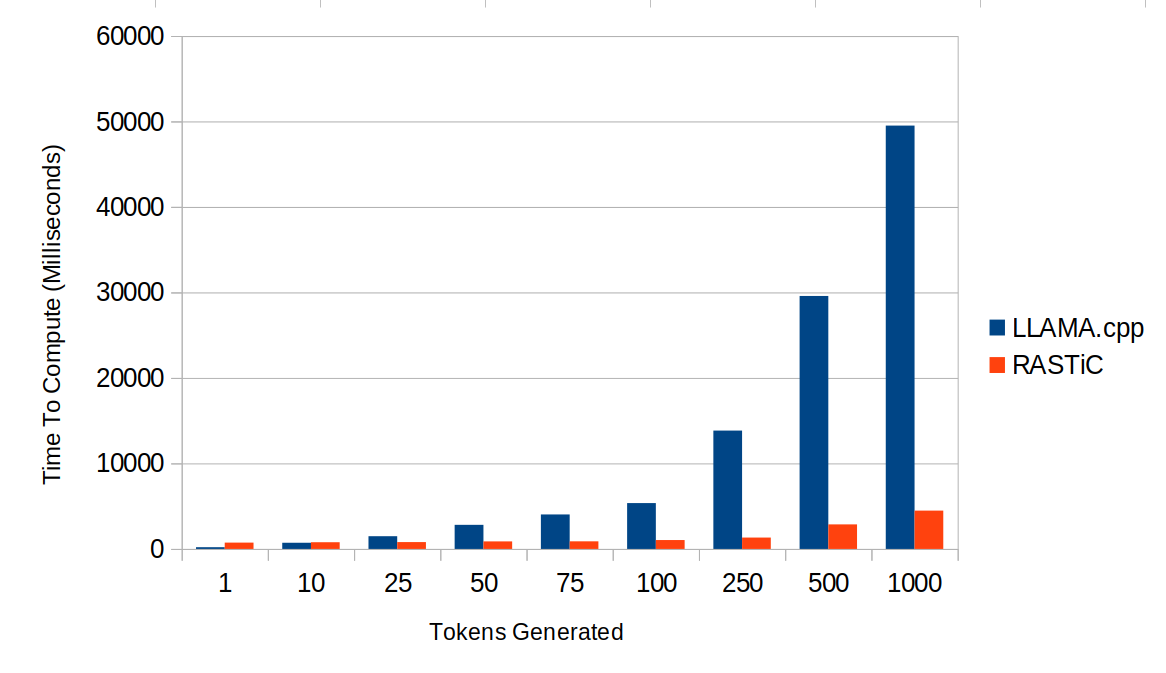
\includegraphics[width=1.0\textwidth]{comparison.png}\par
    \label{fig:comparison}
\end{figure}

As you can see in figure \ref{fig:comparison}, the time required to verify a message using \ac{RASTiC} is significantly less than the time required to generate the message in most cases. 
However, we can see that \ac{RASTiC} is actually slower when verifying messages with fewer than 10 tokens. This is due to the need to tokenize and reload the message into VRAM multiple times.
Custom code could potentially address this issue, but the current lack of libraries with sufficient flexibility hinders such optimizations. 
Future developments should focus on advancing libraries to support these requirements and enhance \ac{RASTiC}'s overall performance.

\subsubsection{Economic Viability}

\paragraph{Enhanced Processing Speeds and GPU Offloading:}
For our testing, we observed greatly increased processing speeds by offloading some layers to the GPU, leveraging the recent innovation of the llama.cpp library. 
This enhancement allowed us to achieve up to 30 tokens per second, even after accounting for overhead. 
Extrapolating these results, we can generate approximately 39,600 tokens per hour under 100\% task saturation.

\paragraph{Cost Analysis and Future Cost Reductions:}
To evaluate the economic viability, we considered the world average cost of electricity, which amounts to \$0.17 per kilowatt hour. 
With a measured average power draw of 312 watts, we calculated the average cost to generate 1000 tokens to be \$0.00134. 
This cost compares favorably to commercial offerings, particularly when considering that certain open-source models approach up to 90\% of the accuracy achieved by OpenAI's GPT models. 
With the adoption of our protocol by users employing specialized and/or dedicated hardware, we anticipate further price reductions, especially as technological innovations continue to improve computation efficiency.

\paragraph{Economic Viability and Conclusion:}
In conclusion, our economic analysis demonstrates the viability of our protocol at a high level. 
The competitive cost per token, combined with the potential for cost reductions and increased demand through hardware adoption and distributed training, establishes a strong foundation for our protocol's economic feasibility. 
Furthermore, the added advantages of privacy and an uncensored user experience further contribute to its value proposition. 
Future developments and advancements in our protocol should solidify its position as a promising solution for efficient LLM generation, training, and verification.

\subsubsection{Rationale}
Sample a subset of the data.
Test for continuity, integrity, and truncation:
\begin{itemize}
    \item \textbf{Continuity:} Ensure that the output is connected to the input. This prevents a case where the output is generated, but is unrelated to the input. 
    This would produce a message where the linkage of tokens is relatively connected, but would be broken at the intersection of the input and output token arrays.
    \item \textbf{Integrity:} Randomly test the interior tokens. 
    Since any one token can be tested it enforces the content of the message to not only be genuinely generated, but also ensures that it hasn't been tampered with since tampering would break every token after it.
    \item \textbf{Truncation:} Ensure that the message has not been truncated. Ensure that an $\langle$end$\rangle$ token has been reached and that the compute note did not prematurely truncate the completion.
\end{itemize}
 With these tests, we can be fairly sure of the integrity of the entire output.


\subsubsection{Potential Attacks and Exploits}

There are a couple of exploits that we can foresee being used to bypass the algorithm.

\begin{enumerate}
    \item \textbf{Repetition:} By using very repetitive outputs, we could theoretically force a false positive. 
    For example, if the tokens for 1 2 3 4 5 6 are seen one after each other, the language model may latch onto the pattern and fill the rest of the output with the pattern, allowing the compute node to bypass expensive computation. 
    However, this is why we test for continuity. 
    Theoretically, the only exploitable inputs would be highly repetitive, and even then, we haven't achieved anything since we can't deviate from the pattern, the pattern that is very close to or identical to truth. 
    However, we do see this as a possible path for exploitation in the future.
    \item \textbf{Trends towards truncation:} While we weren't able to produce an example, sequences could be forced to quickly generate the $\langle$end$\rangle$ token early. 
    However, the node would need to be able to do this more than 51\% of the time or would lose money through slashed stakes.
    \item \textbf{Inference:} Theoretically, because of the limited vocabulary of everyday inputs, lazy prediction algorithms could be used to predict words without use of the official model.
     But, if the node were able to do this effectively enough, this is but an evolution of the network since it would need to be right at least 51\% of the time as not to lose money.
     \item \textbf{Single Token Substitution:} To provide clarity, our testing centers on determining whether significant computational effort was employed in generating the predominant response. 
     This verification approach, however, doesn't offer absolute immunity against single-token substitutions attempted through brute force. 
     Conceivably, a malicious actor could, given sufficient time, alter a single token within the response using brute force. Nevertheless, executing such an endeavor demands substantial resources without any evident financial gain. Our current verification capabilities encompass confirming the utilization of substantial computational resources, in conjunction with the correct model and seed. 
     While the likelihood of this being a concern is minimal, as generating an incorrect response takes longer and elementary substitutions are detectable, we acknowledge it. 
     In most instances, another node will preemptively produce the accurate answer, thereby deterring malicious actions that entail substantial resource investment and risk to staked tokens.
     In an unlikely scenario, a malicious actor could potentially generate a fraction of a response, introduce a random token, and persistently generate the remainder of the response. 
     Detecting such a substitution's occurrence presents odds of 3 in N, where N represents the response's length.
    We could also expect that such a response, if detected by a user, could be flagged for further verification given the financial incentive to do so.
\end{enumerate}

\subsection{Model}
The network will support a diverse range of models, where the term 'Model' encompasses any GPT-like autoregressive model that adheres to the principles of sequential generation. 
A certain level of popularity will be necessary for a model to be considered both usable and secure within the network. 
While participants in the network will have the freedom to host any compatible model of their choice, it is expected that a few highly popular models will dominate the network due to the dynamics of supply and demand. 
The best-performing models, as determined by user demand and overall performance, are likely to attract more usage and attention, solidifying their prominence within the network. 
It is important to note that all models hosted in the network must adhere to the auto-regressive architecture, ensuring that the model's output is generated sequentially based on previously generated tokens. 
The auto-regressive constraint is essential to ensure compatibility with the network's integrity checking algorithm, enabling effective collaboration and optimal utilization of the distributed model infrastructure. 
This requirement guarantees that the model's sequential generation process aligns with the integrity checks performed by the network, ensuring consistent and reliable results across distributed nodes.

\subsubsection{Distribution}
In the distributed architecture, each model, along with its subsequent versions and generations, is identified by its Merkle root. 
This unique identifier ensures integrity and consistency of the model throughout the network.

To store the model, it is divided into small chunks, each having a unique hash. 
These chunks form the building blocks of the model representation. 
The Merkle root is computed by aggregating the hashes of these chunks, providing a concise representation of the entire model.

When a new node joins the network, it can retrieve the model by querying neighboring nodes for the required chunks. 
By requesting chunks in parallel from multiple nodes, the new node can efficiently obtain the complete model.

The Merkle root plays a crucial role in ensuring the authenticity of the model. 
When receiving chunks from neighboring nodes, the new node can verify the integrity of the model by comparing the computed Merkle root with the confirmed Merkle root received from trusted sources. 
This verification process detects any tampering or modification of the model during distribution.

In addition to verifying integrity, the Merkle root is also used to identify and handle invalid chunks. 
By comparing the Merkle root of a received model with the expected Merkle root, the new node can identify any discrepancies and request the necessary chunks again to ensure the model's completeness and correctness.

By leveraging the Merkle root and the distributed storage of model chunks, the network achieves a robust and secure model distribution mechanism.

\section{Key Benefits}
\subsection{Censorship-Proof}
The distributed and open nature of models addresses a challenging issue associated with hosting language models, namely censorship. 
When a single entity hosts a model, they assume the role of the sole arbiter in determining what content is deemed harmful or dangerous. 
Realistically, such entities cannot afford to allow unfiltered text generation, as they bear the responsibility of being publicly accountable. 
However, censorship is a complex task, often resulting in overzealous efforts, as evident in privately held models today. 
These well-intentioned censorship initiatives not only give rise to intricate challenges concerning openness and freedom but also tend to severely restrict current models, rendering them increasingly limited in their usefulness beyond basic tasks.

A distributed and open model offers a democratic approach in determining the capabilities of the model and distributes responsibility in a unique way. 
In such a system, the network serves as a means of facilitating interactions, while individual clients bear the responsibility for their own generations. 
This decentralized structure allows for a collective decision-making process, enabling users to have a say in the model's functionalities and outputs. 
By distributing the blame and accountability across multiple nodes, the network fosters a sense of shared responsibility, minimizing the concentration of power and promoting a more inclusive and democratic environment.

\subsection{Concurrent Inference}
A significant advantage of utilizing a large network of compute nodes is the ability to achieve concurrent inference, enabling multiple inferences to be performed simultaneously. 
Presently, many models are either not designed or are too large to support the computation of multiple inferences on a single client. 
For instance, consider a scenario where an initial query seeks information about the layout of a task, and subsequent inferences aim to provide detailed steps for executing that task. 
With a distributed computing infrastructure, it becomes feasible to handle these subsequent inferences concurrently, greatly enhancing efficiency and responsiveness.

\subsection{Intrinsic Value}
While we refrain from asserting originality in this regard, it's noteworthy that CamelidCoin distinguishes itself from the vast majority of cryptocurrency endeavors through its resource-backed nature. 
In the enduring presence of the network, tokens hold the perpetual potential for exchange in return for computational power. Our network encapsulates a distinctive resource exclusively attainable through this specific coin. 
Each token serves as a certificate for computational resources, akin to a currency backed by gold that maintains the capacity for exchange, thereby carrying the intrinsic value of its representation. 
This intrinsic quality imparts greater resilience to our project in comparison to conventional cryptocurrency protocols.

Unlike the majority of cryptocurrency initiatives, whose value hinges on their potential for appreciation and often evokes a Ponzi scheme dynamic reliant on ever-increasing participation driven by profit aspirations, our approach takes a distinct course. 
viability of other projects tends to wane as hopes for value escalation diminish.
Conversely, the value of our project finds its foundation in representing a unique resource—founded on the ability to be traded for natural language processing. 
This distinctive resource-based valuation model fundamentally distinguishes our initiative, cultivating resilience by connecting tangible utility to our tokens' worth.

\section{Challenges and Limitations}
\subsection{Privacy}
One of the significant challenges with the current protocol is that the inputs must be disclosed to the network, posing a potential privacy risk. 
Although one potential solution is to encrypt the input and wait to disclose it until a node responds, the input must still be disclosed for verification, making it vulnerable to being intercepted by attackers.

A potential solution to this problem is to compute only the first layer of the network before sending it to be completed, which requires only a small slice of the model to be stored locally. 
The averaging of weights and bias in a tensor during this process ensures that there is no way to reconstruct the input, thereby reducing the privacy risk. 
However, this method is not foolproof, as anyone with a copy of the model could finish the computation and access the full unencrypted output.

One approach that has been successful in certain contexts, such as in healthcare, is to hold the last layer of the model secretly by a central authority. 
This approach allows for outsourcing of the majority of the compute without disclosing sensitive information, such as HIPAA data. 
However, this method is not applicable in a fully distributed system, as each node needs a complete copy of the model for verification.

Currently, there is no full model for an auto-regressive zero-knowledge proof, but there are promising fields that may offer alternatives with more research. 
Therefore, privacy remains a significant challenge in the protocol that requires further exploration and development of effective solutions.
\subsubsection{Homomorphic Encryption}
A potential solution to the problem of disclosing inputs in the protocol is the use of homomorphic encryption, which allows for computations to be performed on encrypted data. 
This field of research holds promise for outsourcing auto-regressive models securely. 
However, current developments in fully homomorphic encryption increase the time to compute by several orders of magnitude. 
For instance, encryption operations that can take nanoseconds, such as addition in Paillier encryption, can take several seconds, minutes, or even hours at scale. 
This is not feasible in a distributed neural network computation, where encryption, compute, and decryption must be done within a few seconds. 
Organizations such as OpenMined are leading the effort to implement these principles, but it would require a significant amount of effort and modification to the current model.
\subsection{Inefficient Delegation}
Another challenge with the current implementation is the redundant computation of data, which is a necessary precaution to protect against malicious nodes and account for the ad-hoc nature of the network. 
While this ensures that the quickest free node can respond promptly, it does lead to inefficiencies in the delegation of tasks. 
As a result, there may be opportunities to optimize the process and reduce redundant computation without compromising the integrity of the network. Ongoing research in distributed systems may provide new solutions to this challenge in the future.

\section {Future Aspirations}
\subsection{Distributed Training}
In the process of creating a self-incentivizing economy, we aim to build an enormous collection of compute power. 
With this, we can allow for distributed training of the model, and create regular checkpoints to track progress. 
We believe that nodes will have a strong incentive to contribute to this effort, as the better the model, the more in demand the network will be. 
This will increase the cost per token, which compute nodes can sell back to clients, creating a self-sustaining ecosystem. 
Therefore, we will not need to provide monetary incentives for nodes to participate in this process.

\subsubsection {Federated Averaging}
Federated learning allows for a democratic training process, where the model is shaped by the collective power of the network. 
This allows any data to be slowly incorporated into the model. 
In this process, nodes are free to train any dataset they wish to see incorporated into the model. At set blockchain heights, nodes take time to slow average out their weights with their peers, creating a centralized model which can be agreed upon through several stages of proof of work. 
The specifics of the federated averaging process would need to be explored in detail at a later date.

\subsection{Proof Of Stake}

In the future, we hope to switch over to a proof of stake model. 
This is a challenging task for an emerging coin, as without a large market cap, a minority can take over a large portion of the voting. 
However, once the coin has stabilized and has a sufficient market cap, we plan to follow in the footsteps of Ethereum and make the switch. 
By doing so, we will be able to eliminate the wasteful compute associated with traditional Proof-Of-Work and move towards a more sustainable and eco-friendly system.

While using job completion as proof of work has some potential advantages, it is unlikely to completely replace the proof-of-work algorithm. 
Nevertheless, it is an interesting area of research that could lead to innovative solutions for blockchain scalability and security.

\subsection{Level 2 Payments}
In the future, as the number of transactions continues to increase, the blockchain may face challenges in handling high traffic, low quantity payments efficiently. 
To address this issue, the development of a Level 2 network becomes necessary, which would be built on top of the existing blockchain infrastructure. 
The purpose of this network would be to enable rapid and micro payments.

Layer 2 networks operate by handling thousands of transactions off-chain, utilizing payment channels. 
These channels allow parties to conduct multiple transactions without each individual transaction being recorded on the main blockchain. 
Instead, only the final settlement is recorded, reducing the overall transaction load on the main chain.

To achieve this, Layer 2 networks employ a series of condensing algorithms. 
These algorithms summarize and aggregate the sum of multiple payments made within the payment channels. 
By condensing the information in this way, the need for a record of every single transaction is eliminated, resulting in improved scalability and efficiency.

The introduction of Level 2 payments brings the potential for faster and more scalable transaction processing, making it feasible to handle a large volume of low-value transactions in a more space and cost efficient manner.

\subsection{Task Fractalization}
In the realm of large LLMs, prompt chaining offers a valuable approach to tackling complex problems. 
By breaking down a problem into smaller subtasks, they can be computed individually, overcoming the limitations of smaller models. 
An initial prompt is generated to outline the problem, which then spawns a series of subprompts. 
Instead of completing subtasks sequentially, a network of nodes allows for the parallel computation of subtasks.
For instance, if the goal is to implement the TCP/IP protocol from scratch, which is too complex for any current LLM to handle, an initial task can outline the individual components, and recursively spawn additional jobs or complete when narrow enough in scope.
This technique can be applied to various scenarios, such as querying the network for instructions on creating an eCommerce website.
The initial completion would identify the individual components of an MVC (Model-View-Controller) architecture, such as Users, Products, and Orders.
Each component would then generate subtasks for implementation, such as user registration, user authentication, and user deletion.
This would allow for a feasible one-shot approach to complex task completion.

This fractal like approach to task completion has already been implemented in projects such as AutoGPT. 
However, when run on local language models the time to compute is prohibitively long in some cases, especially on end user hardware which may include smartphones and the like.
By distributing the computation across a network of nodes, the time to compute can be reduced significantly, making it a viable solution for end users.
Tasks of almost infinite complexity could be completed in a time effective manner. Each layer of subtasks only adds 1 additonal time step instead of $n$ time steps, where $n$ is the number of subtasks for a given layer.

\section{Immediate Feasibility of Centralized Implementations}
The implementation of a centralized version of the described network is not only feasible but also highly achievable at present. 
By adopting a centralized approach, the need for a blockchain infrastructure is eliminated, resulting in a significant reduction in complexity.

In this centralized version, the network would rely on a trusted moderator, typically in the form of a company or website, responsible for handling payments and enforcing rules. 
While the network still plays a role in verification, the central authority assumes the tasks of processing payments and administering appropriate penalties. 
To ensure transparency and maintain openness, the actions of the central authority can be justified and made accessible to network participants.

Adopting a centralized model addresses several challenges associated with consensus and blockchain implementation (e.g. inefficiencies related to duplicate task completion). 
For example, the central authority can serve as a task scheduler, strategically assigning tasks to the fastest and most reliable nodes first, keeping more nodes free. 
This approach ensures optimal task allocation, prioritizing faster nodes and balancing workload distribution effectively.


\section {Closing Statements}
Auto-regressive models such as LLMs will define the next decade. Our primary goal is to further democratize large language models.
LLMs have been trained on data created by the collective efforts of humanity and thus belong to the people. 
A concerted effort must be made to prevent LLMs from becoming the exclusive property of monopolistic corporations. 
We believe that large language models should be a force for increasing equity, empowering people from all backgrounds to share and implement their thoughts and ideas without the influence of their ethnic or economic status. 
LLMs are fantastic learning tools that provide access to a wealth of knowledge. 
We are committed to promoting the development of open-source LLM projects and believe that a collective effort can quickly surpass the advancements made by private entities. 
We strive to contribute to the ongoing democratization of language models and work towards a more equitable future for all.

We acknowledge that open source LLM projects have rapidly caught up to those developed by large corporations, and we believe that collective efforts can quickly surpass private ones. 
By fostering an inclusive and collaborative community, we aim to advance the state of the art in auto-regressive models, making them more accessible and beneficial to all.

\end{document}                                                          